\documentclass[11pt, oneside]{article}   	% use "amsart" instead of "article" for AMSLaTeX format
\usepackage{geometry}                		% See geometry.pdf to learn the layout options. There are lots.
\geometry{letterpaper}                   		% ... or a4paper or a5paper or ... 
%\geometry{landscape}                		% Activate for for rotated page geometry
%\usepackage[parfill]{parskip}    		% Activate to begin paragraphs with an empty line rather than an indent
\usepackage{graphicx}				% Use pdf, png, jpg, or eps� with pdflatex; use eps in DVI mode
								% TeX will automatically convert eps --> pdf in pdflatex		
\usepackage{amssymb}
\graphicspath{{/Users/telliott_admin/Dropbox/Tex/png/}}

\title{Derivative of sine and cosine}
%\author{The Author}
\date{}							% Activate to display a given date or no date

\begin{document}
\maketitle
%\section{}
%\subsection{}
\large
As we saw before, the derivative of the function $f(x)$ is defined to be
\[ \lim_{h \to 0}  \  \frac{f(x+h) - f(x)}{h}  \]
What if $f(x) = sin \ x$?  Just follow the pattern.  The difference quotient is
\[ \frac{sin(x + h) - sin \ x}{h} \]
We expand the first term using the sum of angles formula
\[ \frac{sin \ x \ cos \ h + cos \ x \ sin \ h - sin \ x}{h} \]
Group the terms with $sin \ x$ together
\[ sin \ x \ (\frac{cos \ h - 1}{h}) + cos \ x (\frac{sin \ h}{h} ) \]
We will show that
\[ \lim_{h \to 0} \   \frac{cos \ h - 1}{h}  = 0 \]
\[ \lim_{h \to 0} \   \frac{sin \ h}{h}   = 1 \]
so that 
\[ \frac{d}{dx}( sin \ x) = \lim_{h \to 0} \ sin \ x \ (\frac{cos \ h - 1}{h}) + cos \ x (\frac{sin \ h}{h} ) =  cos \ x \]
For the cosine, the difference quotient is
\[ \frac{cos(x + h) - cos \ x}{h} \]
We again expand the first term using the sum of angles formula
\[ \frac{cos \ x \ cos \ h - sin \ x  \ sin \ h - cos \ x}{h} \]
Now we group the terms with $cos \ x$ togther
\[ cos \ x (\frac{cos \ h - 1}{h}) - sin \ x (\frac{sin \ h}{h} ) \]
Using the same limits as before, we obtain
\[ \frac{d}{dx}( cos \ x) = \lim_{h \to 0} \ cos \ x (\frac{cos \ h - 1}{h}) - sin \ x (\frac{sin \ h}{h}) =  - sin \ x \]
So now, we need to find those limits.  Start with 
\[ \lim_{h \to 0} \   \frac{sin \ h}{h}   = 1 \]
\begin{center}
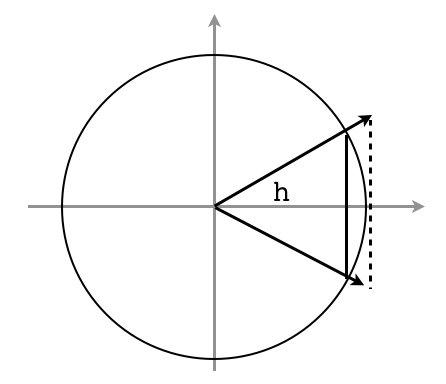
\includegraphics [scale=0.5] {sine_limit.png}
\end{center}
We draw the angle $h$ above and below the x-axis on the unit circle (radius equal to 1).  The solid vertical line is a secant of the circle, the part above the x-axis is equal to $sin \ h$.  Since it is a secant, and a line is the shortest distance between two points, that length is always less than the length of the arc of the circle, when $h \to 0$.  Considering just the part above the x-axis, we have that
\[ sin \ h < h \]
The dotted line is twice the tangent of $h$, and the part above the x-axis is equal to the $tan \ h$.  As long as $h > 0$, the area of the triangle with $tan \ h$ as its side will be greater than the slice of the circle with arc length $h$.  We have
\[ sin \ h < h < tan \ h \]
Divide by $sin \ h$
\[ 1 < \frac{h}{sin \ h} < \frac{1}{cos \ h} \]
As $h \to 0$, $cos \ h \to 1$ so
\[ 1 < \frac{h}{sin \ h} < 1 \]
The ratio $\frac{h}{sin \ h}$ gets "squeezed" between two other terms that go to 1, so it  must also be equal to 1 in the limit.
For the other limit
\[ \lim_{h \to 0} \   \frac{cos \ h - 1}{h}  = 0 \]
multiply top and bottom
\[ \frac{cos \ h - 1}{h} \  (\frac{cos \ h + 1}{cos \ h + 1}) =  \frac{cos^2 h - 1}{h (cos \ h + 1)} = \frac{-sin^2h}{h(cos \ h + 1)} = \frac{-sin \ h}{h} \ \frac{sin \ h}{cos \ h + 1} \]
In the limit as $h \to 0$, the left term is equal to 1 (with a minus sign), as we just saw.  The right-hand term is
\[ \frac{sin \ h}{cos \ h + 1} \] 
As $h \to 0$, the numerator goes to 0 and the denominator goes to 1, so this term is equal to 0, and therefore the whole thing is equal to 0.

We should not let all this business about limits obscure the simplicity of the basic result:
\[ \frac{d}{dx}( sin \ x) = cos \ x \]
\[ \frac{d}{dx}( cos \ x) = -sin \ x \]

\end{document}  